\chapter{PHÂN TÍCH HỆ THỐNG}
Pha phân tích mô tả hệ thống phải làm gì để đáp ứng yêu cầu: mục tiêu của tác nhân, hành vi, các khái niệm miền và trách nhiệm phối hợp. Phần này chưa quyết định cấu trúc router, kiểu lưu trữ hay hợp đồng HTTP; các lựa chọn đó được cụ thể hóa ở Chương 4.

\section{Mô hình use case tổng quát và phân hệ}
Mã UC01--UC34 được giữ để truy vết về đặc tả hiện có. Sơ đồ tổng quát chỉ trình bày các mục tiêu chính; \textbf{10 sơ đồ PK01--PK10 trong phụ lục} bao phủ đủ 34 UC. Không nhồi tất cả actor, oval và cạnh lên một hình khiến không đọc được.

{\footnotesize\setlength{\tabcolsep}{0pt}
\begin{longtable}{@{}L{5.133cm}@{\hspace{3mm}}L{5.133cm}@{\hspace{3mm}}L{5.133cm}@{}}
\caption{Mô hình use case tổng quát và phân hệ}\\
\toprule
\textbf{Phân hệ} & \textbf{Use case} & \textbf{Vai trò chính} \\
\midrule\endfirsthead
\multicolumn{3}{l}{\small\itshape Bảng \thetable{} (tiếp theo)}\\
\toprule
\textbf{Phân hệ} & \textbf{Use case} & \textbf{Vai trò chính} \\
\midrule\endhead
\bottomrule\endfoot
PK1 Tài khoản và bảo mật & UC01 đăng ký; UC02 đăng nhập; UC03 đăng xuất; UC04 đặt lại mật khẩu & A01, A02 \\ \addlinespace[3pt]
PK2 Quyền riêng tư & UC05 quản lý đồng ý; UC06 tải dữ liệu; UC07 xóa tài khoản; UC08 yêu cầu sửa/\allowbreak{}hạn chế/\allowbreak{}phản đối & A02, A04 hỗ trợ \\ \addlinespace[3pt]
PK3 Hồ sơ và mục tiêu & UC09 thiết lập hồ sơ; UC10 cập nhật hồ sơ/\allowbreak{}dị ứng/\allowbreak{}bếp; UC11 đặt mục tiêu năng lượng & A02 \\ \addlinespace[3pt]
PK4 Kho và quét & UC12 quét ảnh; UC13 sửa/\allowbreak{}xác nhận kết quả; UC14 quản lý kho theo lô & A02 \\ \addlinespace[3pt]
PK5 Mâm cơm & UC15 nhận mâm; UC16 đổi món; UC17 chọn thay thế; UC18 quản lý danh sách đi chợ & A02 \\ \addlinespace[3pt]
PK6 Nấu và nhật ký & UC19 nấu cả mâm; UC20 hoàn tất; UC21 hoàn tác; UC22 nhật ký tuần & A02 \\ \addlinespace[3pt]
PK7 Khảo sát gu & UC23 tham gia khảo sát; UC24 quản lý đợt khảo sát & A03, A06 \\ \addlinespace[3pt]
PK8 Nội dung và dữ liệu & UC25 nhập kho công thức; UC26 cặp thay thế; UC27 xử lý yêu cầu dữ liệu/\allowbreak{}kiểm toán & A05, A04 \\ \addlinespace[3pt]
PK9 Vận hành mô hình & UC28 xuất dữ liệu huấn luyện; UC29 đăng ký/\allowbreak{}kiểm định; UC30 triển khai/\allowbreak{}quay lui; UC31 gán nhãn & A06, A07, A10 \\ \addlinespace[3pt]
PK10 Tác vụ định kỳ & UC32 xóa ảnh quá hạn; UC33 sao lưu; UC34 dọn job/\allowbreak{}token/\allowbreak{}khóa hết hạn & A08 \\ \addlinespace[3pt]
\end{longtable}}
\begin{figure}[H]\centering
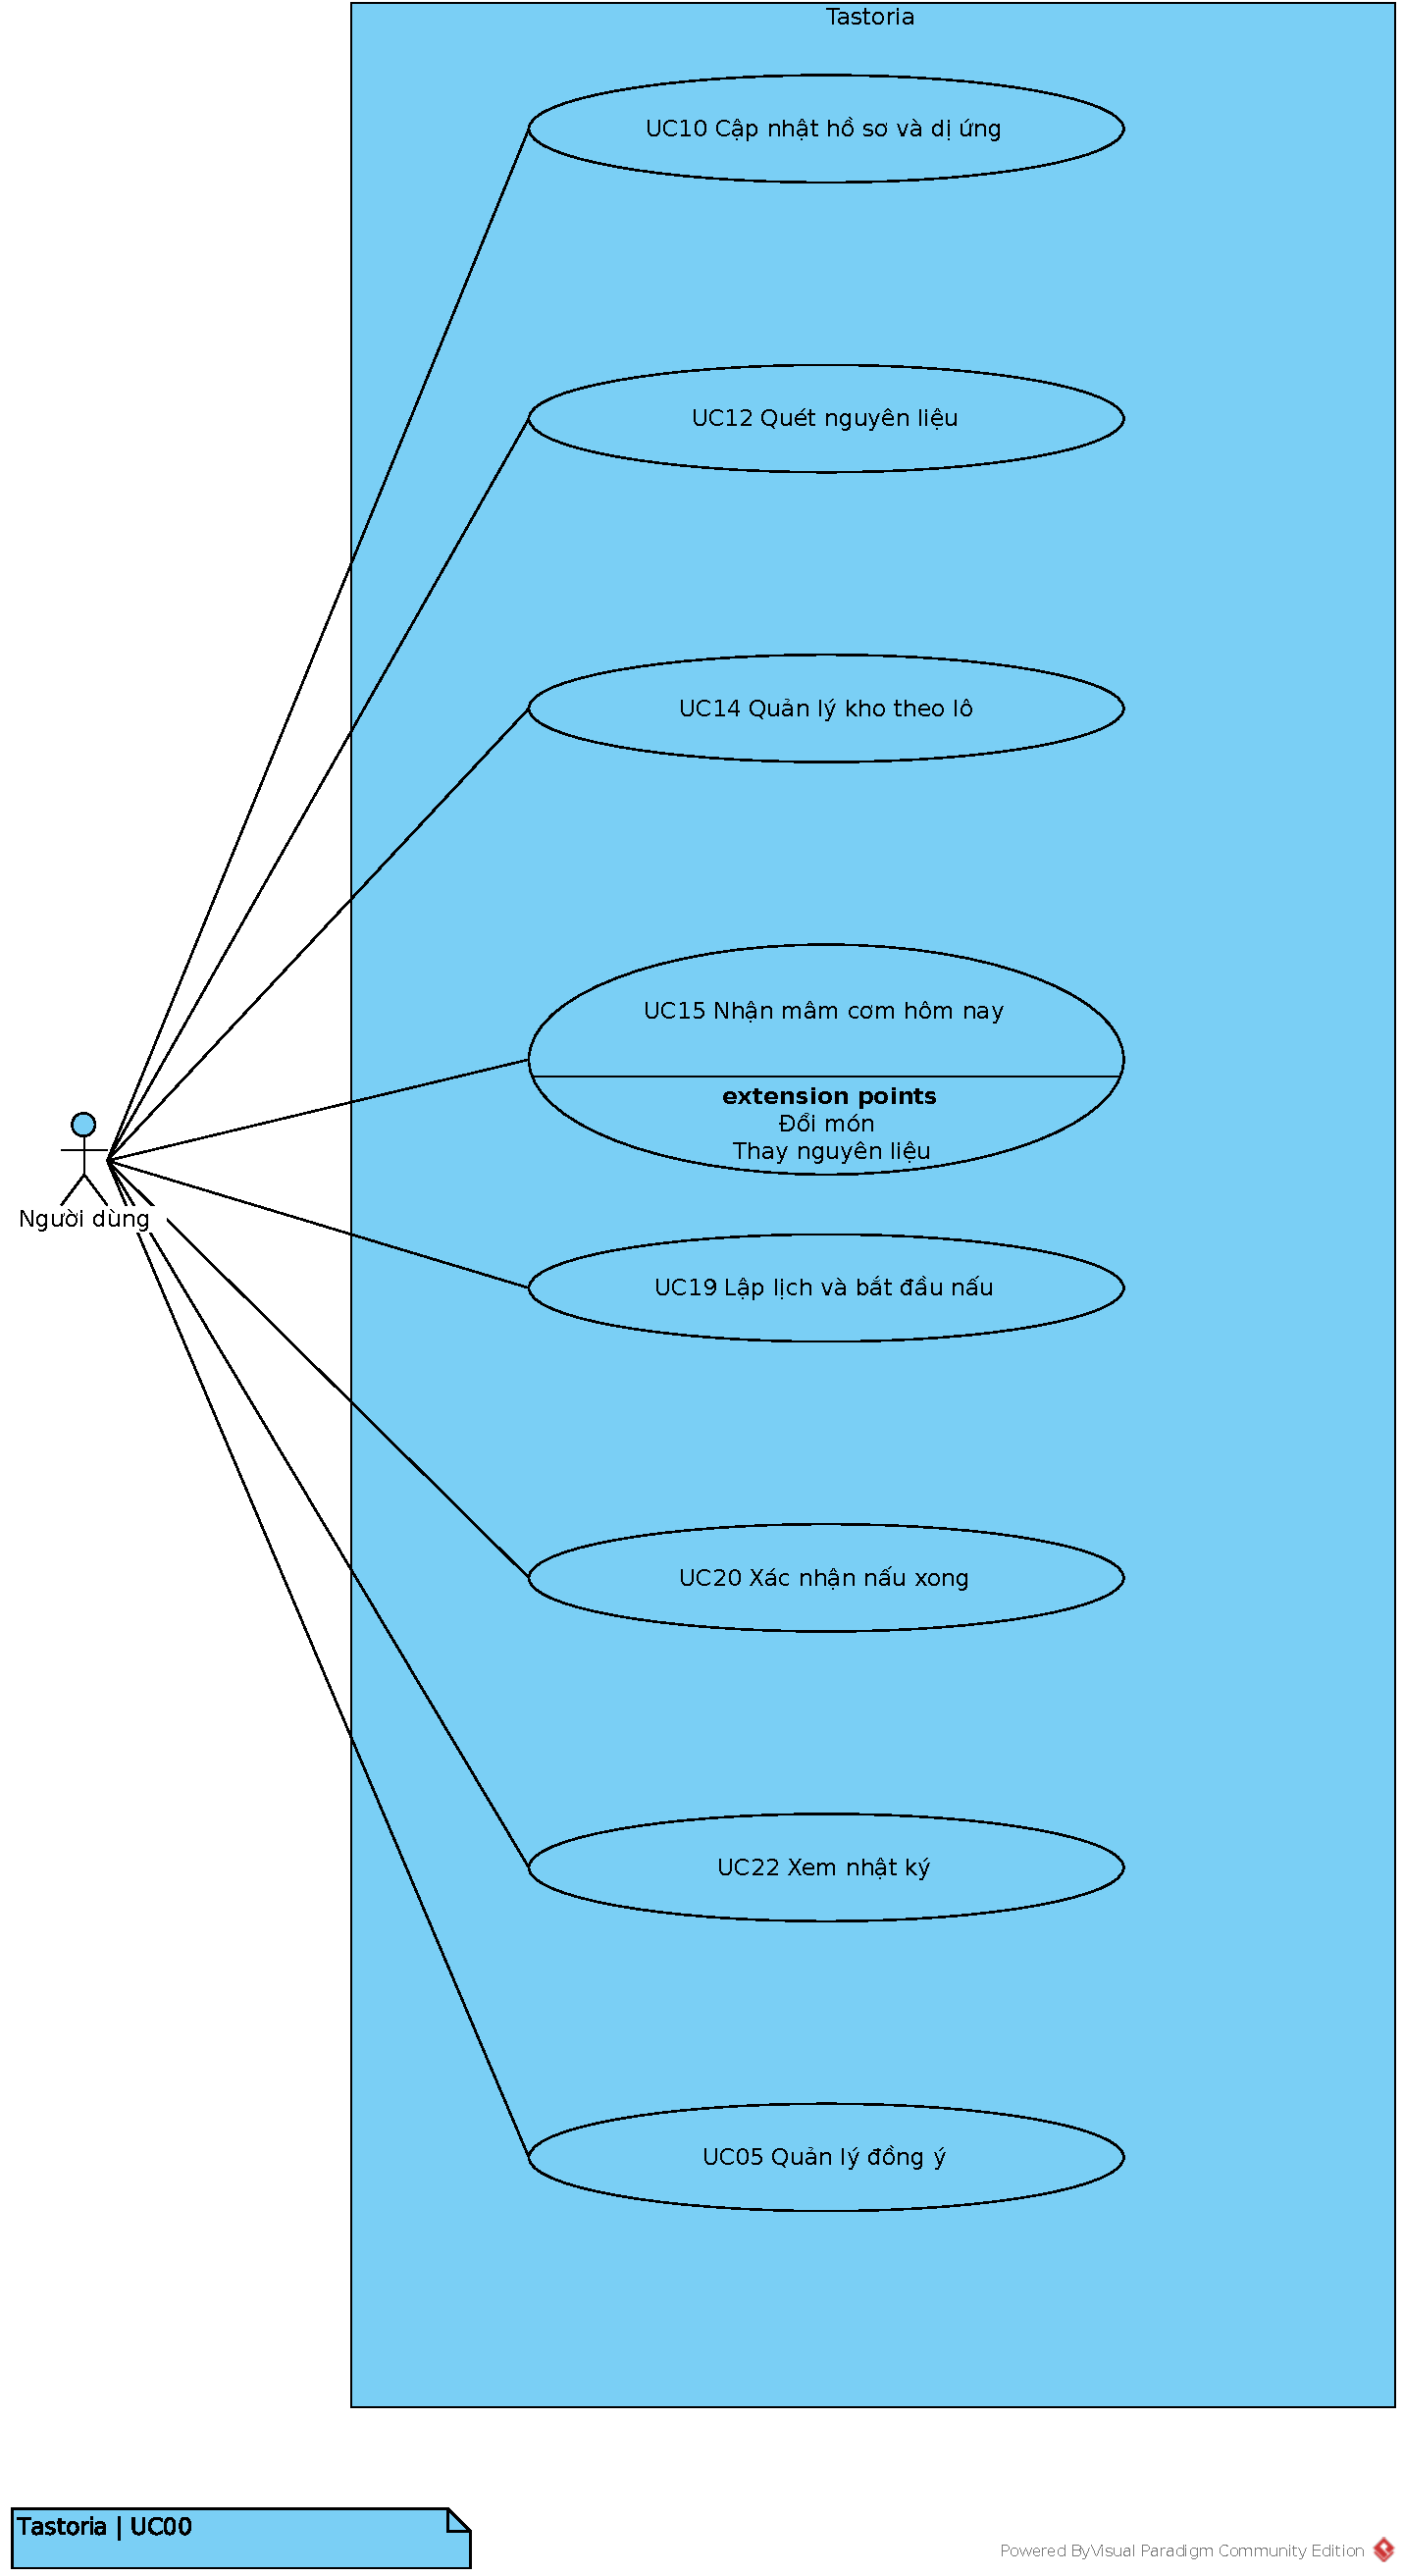
\includegraphics[width=0.96\linewidth,height=0.75\textheight,keepaspectratio]{assets/UC00.pdf}
\caption{UC00 --- Các mục tiêu chính của người nấu}\label{fig:Bao-cao-Tastoria:1}
\end{figure}
\textbf{Quy tắc đọc sơ đồ:} đường actor--UC là association, không biểu diễn thứ tự. {\small\texttt{extend}} hướng từ UC mở rộng về UC cơ sở, có điểm mở rộng và điều kiện. {\small\texttt{include}} chỉ dùng khi hành vi được gọi bắt buộc, không dùng để biểu diễn ``màn hình sau'' hay ``phải đăng nhập trước''. Không tạo kế thừa actor chỉ vì hai vai trò có chung một màn hình.

\section{Phân tích quan hệ use case}
{\footnotesize\setlength{\tabcolsep}{0pt}
\begin{longtable}{@{}L{5.133cm}@{\hspace{3mm}}L{5.133cm}@{\hspace{3mm}}L{5.133cm}@{}}
\caption{Phân tích quan hệ use case}\\
\toprule
\textbf{Quan hệ trong tài liệu cũ} & \textbf{Phân tích lại} & \textbf{Cách trình bày ở bản này} \\
\midrule\endfirsthead
\multicolumn{3}{l}{\small\itshape Bảng \thetable{} (tiếp theo)}\\
\toprule
\textbf{Quan hệ trong tài liệu cũ} & \textbf{Phân tích lại} & \textbf{Cách trình bày ở bản này} \\
\midrule\endhead
\bottomrule\endfoot
UC12 include UC13 & UC12 kết thúc khi có kết quả nhận diện; người dùng có thể bỏ kết quả mà không nhập kho & Hai mục tiêu liên tiếp trong activity. UC13 là thao tác xác nhận riêng, không include bắt buộc từ nhận diện \\ \addlinespace[3pt]
UC09 include UC05 & Việc quản lý đồng ý là mục tiêu riêng; phần khai sức khỏe có thể được bỏ qua & Mô tả điều kiện đồng ý trong luồng UC09 và BR; không include toàn bộ ``quản lý đồng ý'' \\ \addlinespace[3pt]
UC16/\allowbreak{}UC17 extend UC15 & Có ý nghĩa nếu UC15 bao gồm xem và điều chỉnh mâm đề xuất & Giữ extend với hai điểm ``Đổi món'' và ``Thay nguyên liệu'' trong lúc xem mâm; điều kiện là người dùng chủ động yêu cầu \\ \addlinespace[3pt]
UC18 extend UC15/\allowbreak{}UC17 & Danh sách đi chợ tồn tại và được quản lý độc lập, không chỉ trong lúc nhận mâm & Association từ người dùng tới UC18; thêm nguyên liệu thiếu là luồng tùy chọn của UC15/\allowbreak{}UC17 \\ \addlinespace[3pt]
UC21 extend UC20 & Hoàn tác diễn ra sau giao dịch hoàn tất đã kết thúc & UC21 độc lập, tiền điều kiện là phiên đã hoàn tất và còn hạn; sequence thể hiện giao dịch đảo \\ \addlinespace[3pt]
\end{longtable}}
Đây là điều chỉnh mô hình trong báo cáo, không tự sửa bộ đặc tả gốc hoặc thay đổi hành vi phần mềm. Nhóm cần thống nhất phiên bản khi hợp nhất lại {\small\texttt{model.\allowbreak{}yaml}}.

\clearpage\begin{landscape}
\begin{figure}[H]\centering
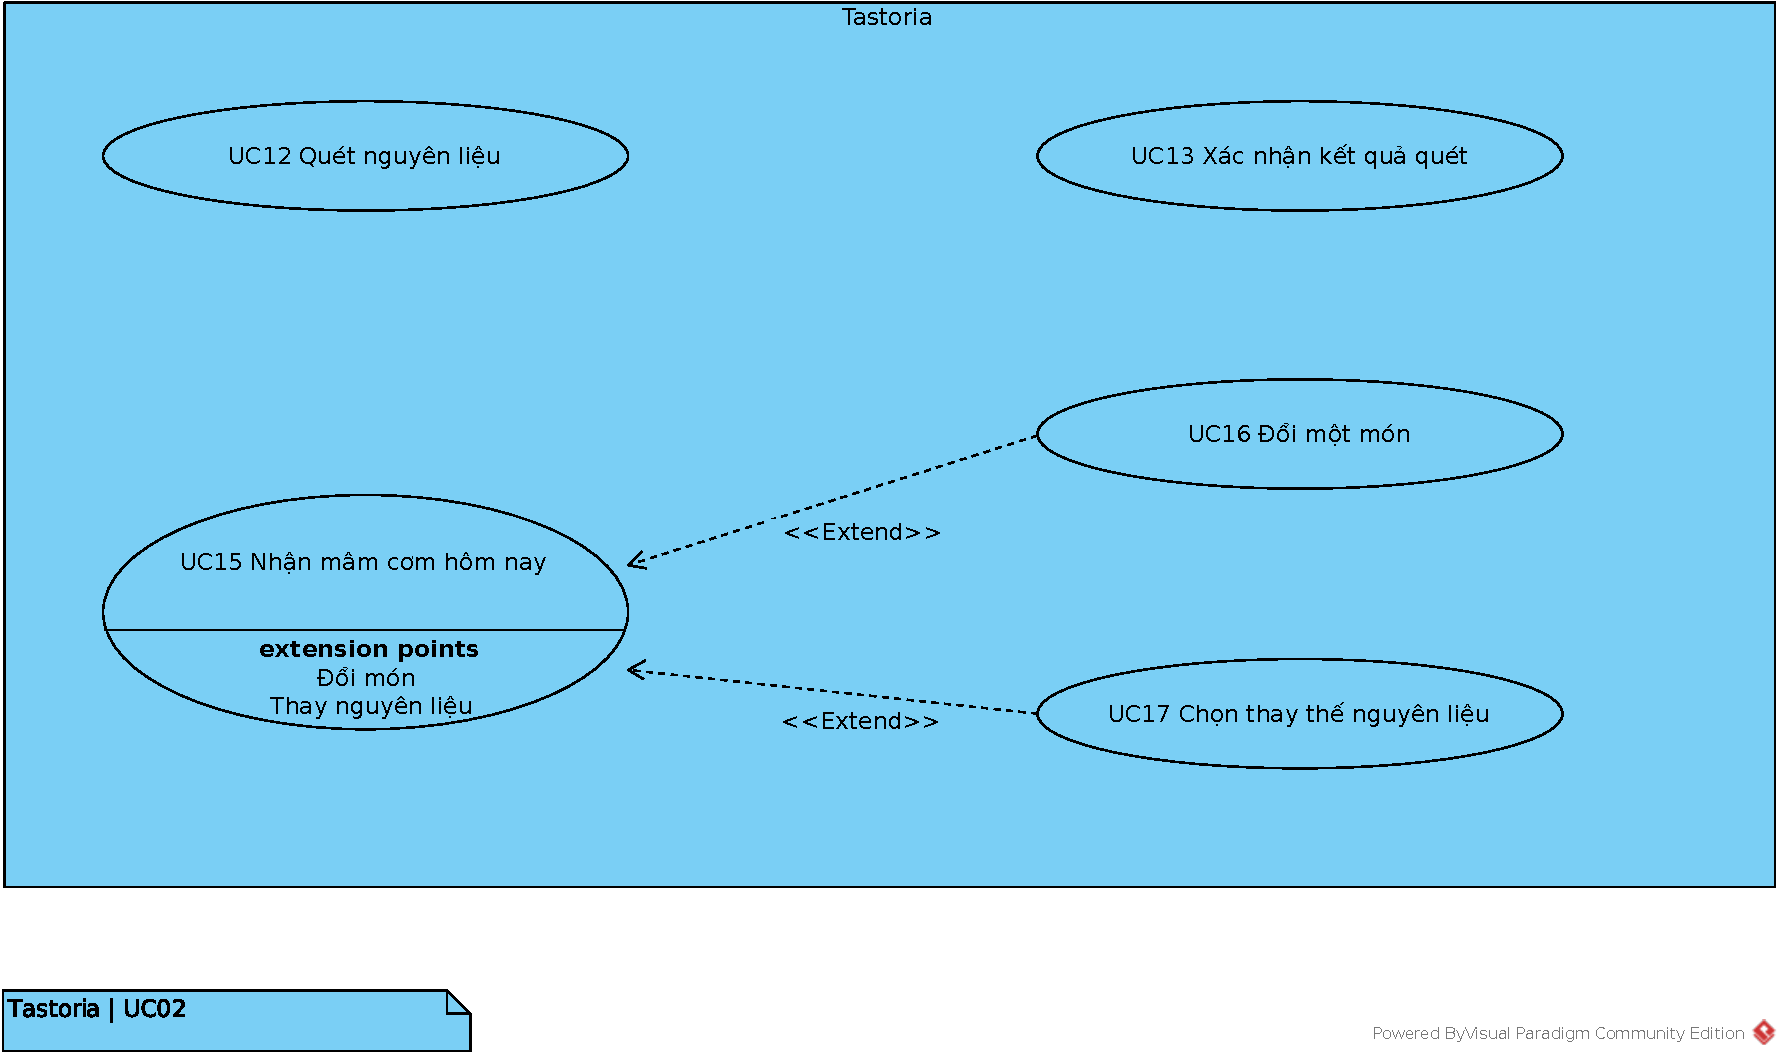
\includegraphics[width=0.96\linewidth,height=0.78\textwidth,keepaspectratio]{assets/UC02.pdf}
\caption{UC02 --- Mở rộng khi xem mâm; không nối quét và xác nhận bằng include}\label{fig:Bao-cao-Tastoria:2}
\end{figure}
\end{landscape}\clearpage
\section{Đặc tả và hợp đồng nghiệp vụ}
UC tổng quát thể hiện mục tiêu có giá trị cho tác nhân. Sơ đồ PK phân nhóm các mục tiêu đó theo trách nhiệm; không phải cứ nằm trong cùng phân hệ thì các UC có quan hệ include. Các thao tác kỹ thuật như kiểm JWT, khóa bản ghi và commit là trách nhiệm thiết kế, không tách thành UC người dùng chỉ để làm sơ đồ nhiều nút hơn.

Phụ lục A giữ đủ 34 đặc tả. Với từng UC, người đọc cần xác định được: ai kích hoạt, dữ liệu/\allowbreak{}trạng thái nào phải có trước, luồng thành công, vị trí rẽ nhánh, dữ liệu thay đổi và dữ liệu phải giữ nguyên khi thất bại. Các mục tiêu trọng tâm được phân tích tiếp trong các mục tiếp theo: UC09--10, UC13, UC15, UC20--21 và UC30. Những UC còn lại có đặc tả đầy đủ nhưng chưa có một bộ activity/\allowbreak{}sequence/\allowbreak{}lớp riêng cho từng UC; phạm vi này được công khai trong bảng truy vết.

{\footnotesize\setlength{\tabcolsep}{0pt}
\begin{longtable}{@{}L{2.960cm}@{\hspace{3mm}}L{2.960cm}@{\hspace{3mm}}L{2.960cm}@{\hspace{3mm}}L{2.960cm}@{\hspace{3mm}}L{2.960cm}@{}}
\caption{Đặc tả và hợp đồng nghiệp vụ}\\
\toprule
\textbf{UC trọng tâm} & \textbf{Tiền điều kiện} & \textbf{Điểm quyết định} & \textbf{Hậu điều kiện thành công} & \textbf{Bảo đảm khi lỗi} \\
\midrule\endfirsthead
\multicolumn{5}{l}{\small\itshape Bảng \thetable{} (tiếp theo)}\\
\toprule
\textbf{UC trọng tâm} & \textbf{Tiền điều kiện} & \textbf{Điểm quyết định} & \textbf{Hậu điều kiện thành công} & \textbf{Bảo đảm khi lỗi} \\
\midrule\endhead
\bottomrule\endfoot
UC13 Xác nhận quét & Lần quét thuộc người gọi, trạng thái done & Lượng bắt buộc, mục đã xóa, trạng thái gửi lại & Kho và scan confirmed cùng được ghi & Không để kho thay đổi mà scan vẫn chưa xác nhận \\ \addlinespace[3pt]
UC15 Nhận mâm & Người dùng có bối cảnh hợp lệ & Dị ứng, lượng chung, thời gian, ứng viên khả thi & Mâm đề xuất có món, khẩu phần và lý do & Không tạo mâm giả bằng cách âm thầm bỏ ràng buộc cứng \\ \addlinespace[3pt]
UC20 Hoàn tất & Phiên thuộc người gọi & in\_\allowbreak{}progress, completed hoặc trạng thái không hợp lệ & Giao dịch kho, phiên completed, mâm cooked nhất quán & Retry không trừ lại; lỗi trước commit không để trạng thái dở dang \\ \addlinespace[3pt]
UC21 Hoàn tác & Phiên đã completed và còn thời hạn & Thời gian máy chủ; phiên reverted gửi lại & Ghi đảo, phiên reverted, mâm accepted & Không đảo ngoài hạn hoặc đảo lần hai \\ \addlinespace[3pt]
UC30 Triển khai & Vai trò vận hành và phiên bản được phép chọn & Tính tương thích artifact, ánh xạ lớp và trạng thái kiểm định & Chọn phiên bản hoạt động có khả năng truy vết & Không dùng tên phiên bản thay cho bằng chứng chất lượng \\ \addlinespace[3pt]
\end{longtable}}
\section{Phân tích luồng nghiệp vụ và ngoại lệ}
Các luồng dưới đây chọn theo mục tiêu nghiệp vụ, không theo người thực hiện bài tập. AD01--AD02 mô tả luồng thành công; AD03 và các bảng ngoại lệ bổ sung điều kiện quyết định. Đặc tả đầy đủ được giữ ở Phụ lục A.

\subsection{Tài khoản, hồ sơ và quyền dữ liệu}
Phạm vi UC01--UC11. Khách đăng ký bằng email/\allowbreak{}mật khẩu; đăng nhập thành công mở vùng bếp. Người dùng thiết lập dị ứng, chế độ ăn, số bếp và mục tiêu; chỉ thu thập dữ liệu nhạy cảm khi có đồng ý thích hợp. Rút đồng ý không đồng nghĩa xóa toàn bộ tài khoản; xóa tài khoản là quy trình riêng.

Ngoại lệ cần phân biệt: email đã dùng, mật khẩu không hợp lệ, đăng nhập sai/\allowbreak{}quá giới hạn, refresh token hết hạn hoặc bị dùng lại, dữ liệu hồ sơ không hợp lệ, yêu cầu dữ liệu không thuộc người gọi. Lỗi không được lộ dữ liệu tài khoản người khác. Xem phụ lục UC01--UC11 để đọc tiền/\allowbreak{}hậu điều kiện và FR gốc.

\subsection{Quét ảnh và quản lý kho theo lô}
UC12--UC14. Người dùng chọn chế độ toàn tủ hoặc đồ vừa mua, tải 1--2 ảnh, theo dõi xử lý, sửa chip nguyên liệu và xác nhận. Chỉ bước xác nhận ghi kho; cùng ngăn có quy tắc gộp tránh đếm lặp. Quét toàn tủ có thể đánh dấu lô không thấy để người dùng kiểm, không tự xóa.

Luồng thất bại: không cấp quyền ảnh \ensuremath{\rightarrow} nhập tay; ảnh sai định dạng/\allowbreak{}dung lượng \ensuremath{\rightarrow} sửa đầu vào; worker lỗi \ensuremath{\rightarrow} retry giới hạn rồi báo thất bại; mất mạng \ensuremath{\rightarrow} hỏi lại mã scan; bỏ kết quả \ensuremath{\rightarrow} không đổi kho; xác nhận lặp \ensuremath{\rightarrow} không thêm lô trùng.

\begin{figure}[H]\centering
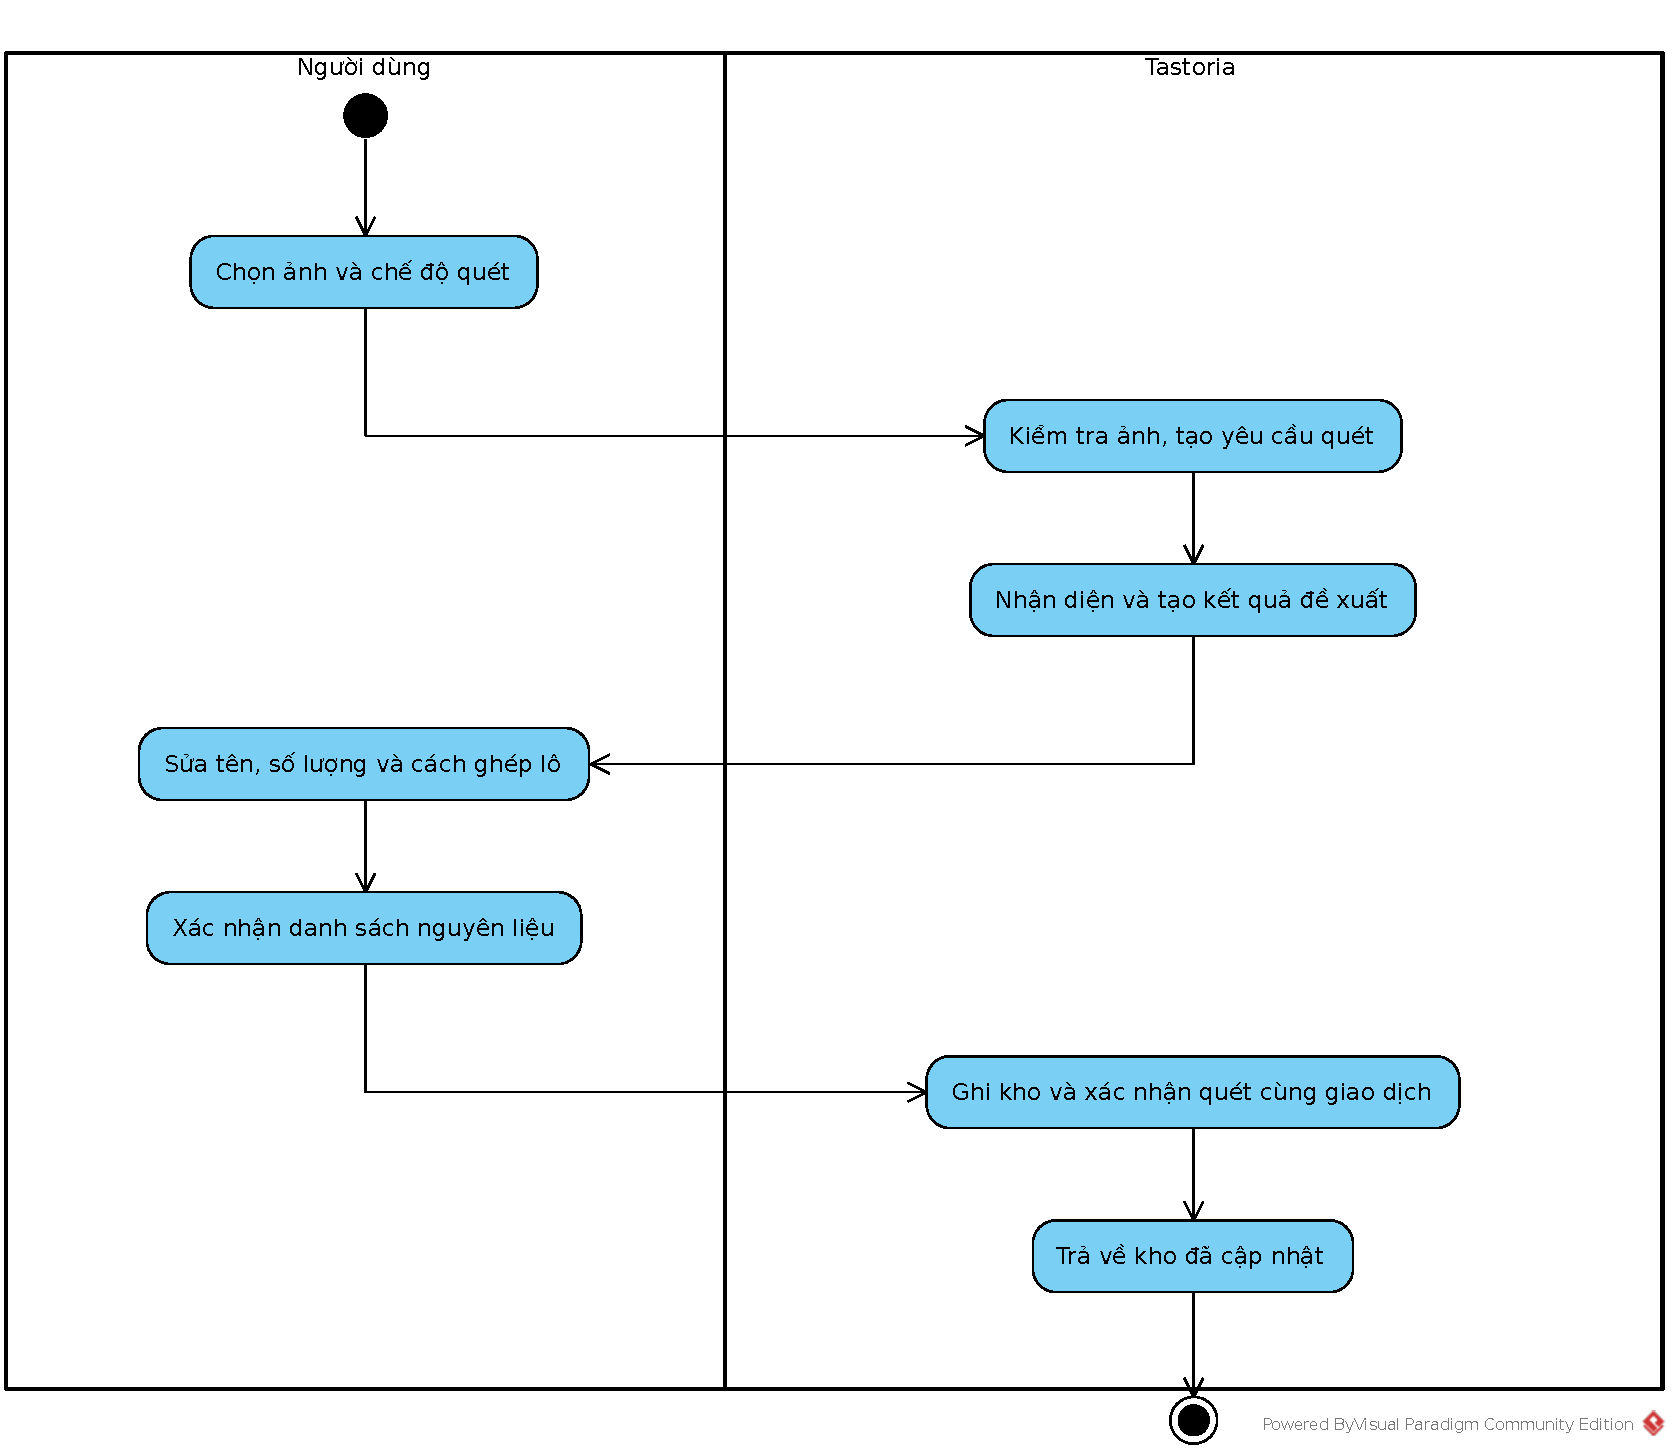
\includegraphics[width=0.96\linewidth,height=0.75\textheight,keepaspectratio]{assets/AD01.pdf}
\caption{AD01 --- Luồng thành công quét và xác nhận; các ngoại lệ xem đặc tả UC12--UC14}\label{fig:Bao-cao-Tastoria:3}
\end{figure}
\subsection{Gợi ý mâm, đổi món và đi chợ}
UC15--UC18. Nhập số người, thời gian, dị ứng người ăn cùng và lô ưu tiên. Hệ thống loại món không hợp lệ, tính lượng theo khẩu phần, ghép tổ hợp, kiểm tổng nhu cầu và thời gian rồi xếp hạng. Người dùng xem lý do, đổi một món hoặc chọn thay thế hợp lệ trước khi chấp nhận.

Không có mâm khả thi phải báo thiếu gì hoặc đề xuất thay đổi điều kiện, không âm thầm bỏ ràng buộc dị ứng. Đổi món cố định các vị trí còn lại nhưng vẫn tính lại toàn mâm. Thêm thứ cần mua không được coi như nguyên liệu đã có trong kho.

\begin{figure}[H]\centering
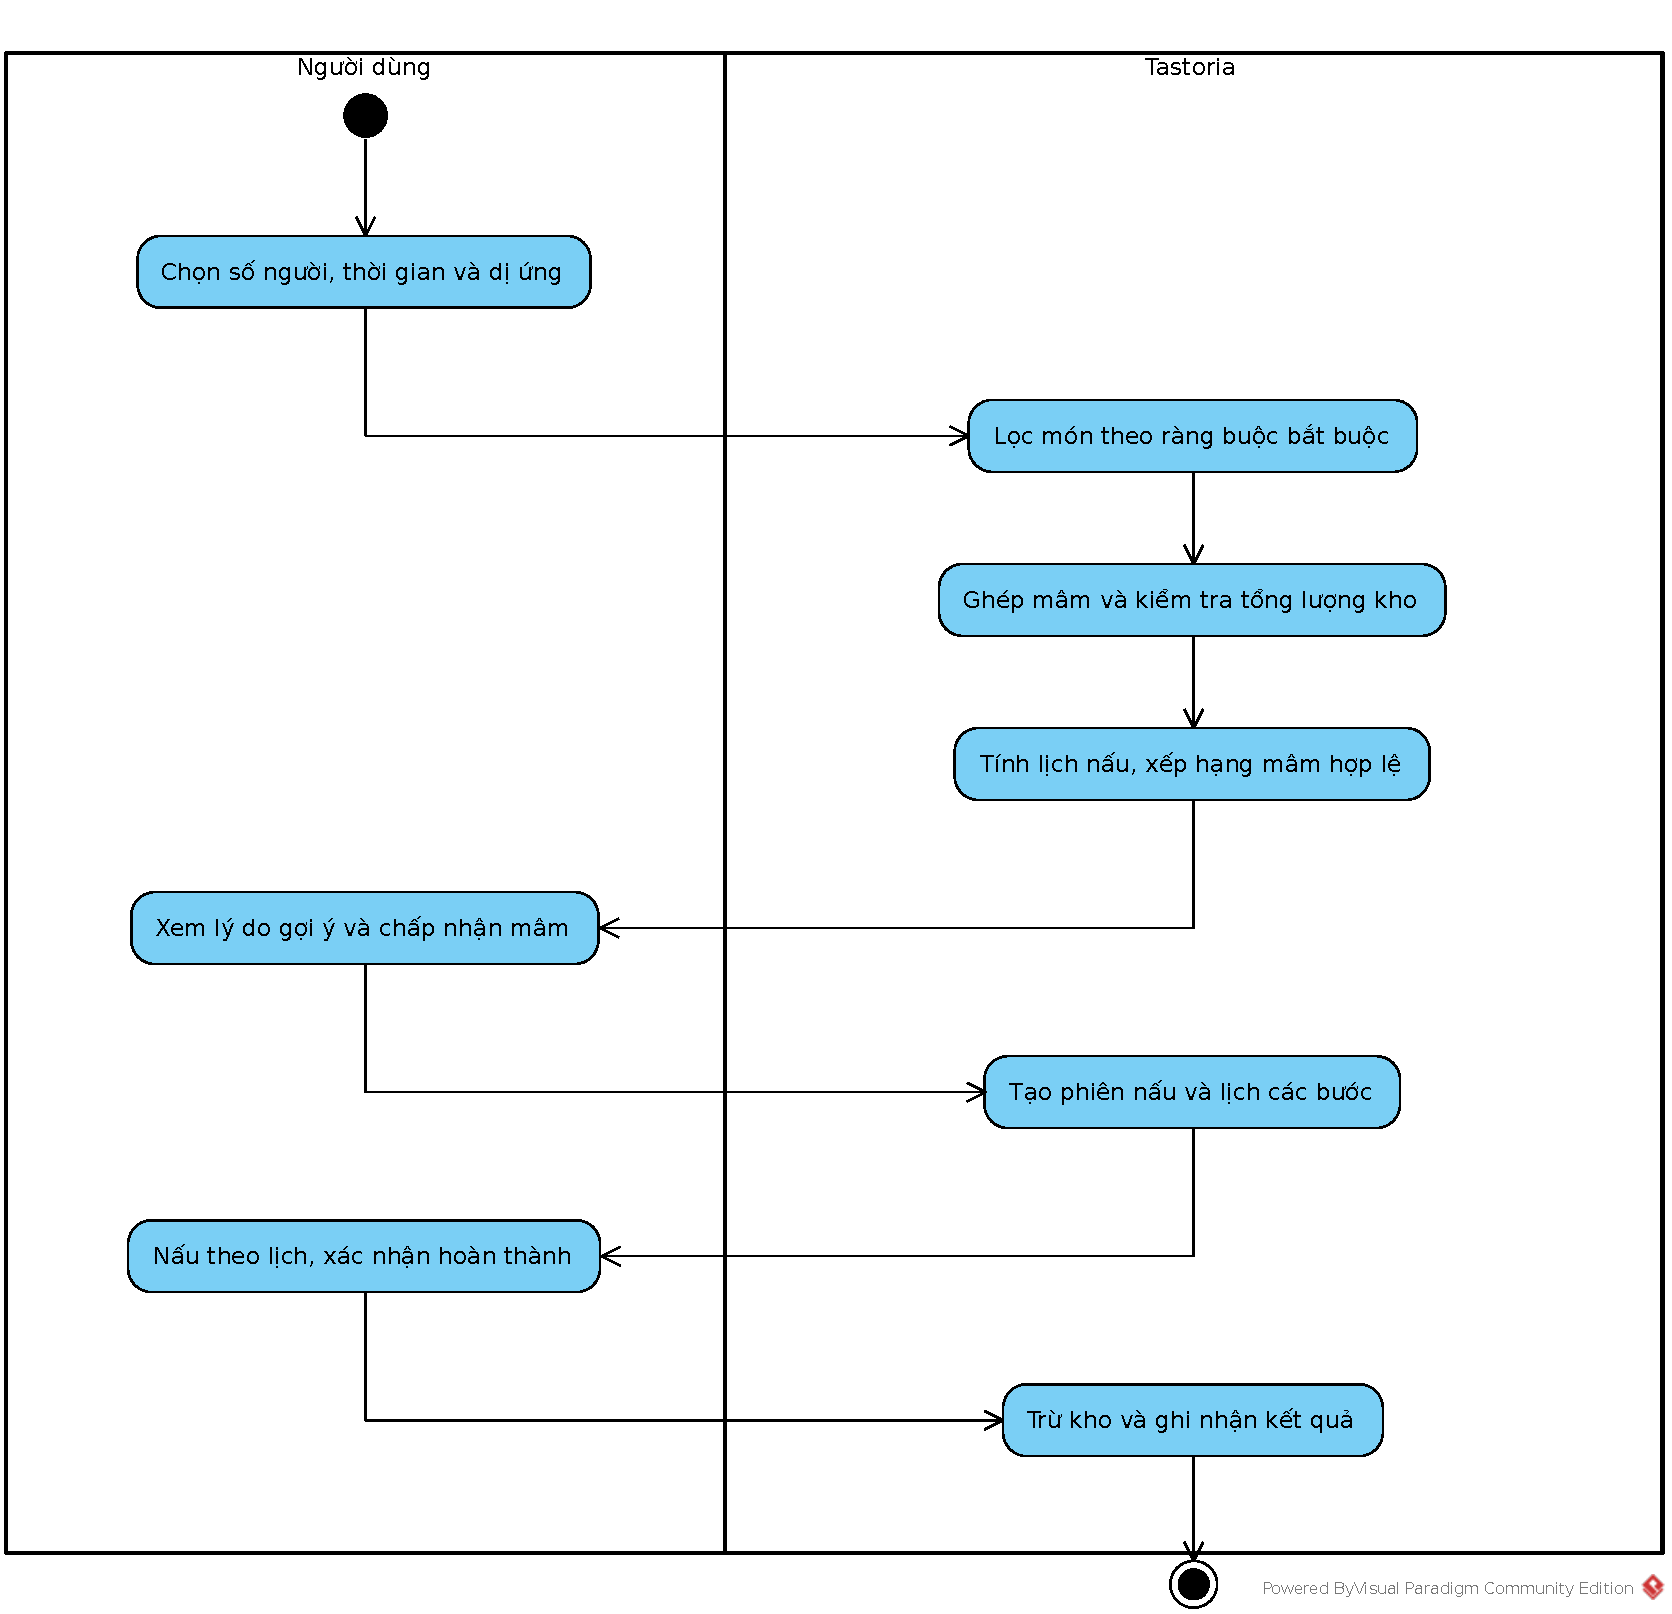
\includegraphics[width=0.96\linewidth,height=0.75\textheight,keepaspectratio]{assets/AD02.pdf}
\caption{AD02 --- Luồng thành công từ yêu cầu mâm đến hoàn tất}\label{fig:Bao-cao-Tastoria:4}
\end{figure}
\subsection{Lịch nấu, hoàn tất, hoàn tác và nhật ký}
UC19--UC22. Mâm được chấp nhận mới tạo phiên nấu. Lịch xét thứ tự bước, thao tác chủ động và số bếp. Khi nấu xong, người dùng đánh giá tùy chọn và xác nhận. Hệ thống trừ kho một lần, cập nhật phiên/\allowbreak{}mâm; hoàn tác trong 10 phút bằng giao dịch đảo. Nhật ký dựa trên dữ liệu đã hoàn tất, không đếm lại một request retry.

Bộ lịch có thể nới điều kiện các món xong gần nhau hoặc trả lịch tuần tự dự phòng; không nới số bếp và thứ tự công việc để tạo lịch giả. Khi mất mạng, outbox giữ yêu cầu hoàn tất và cùng khóa lũy đẳng để gửi lại.

\clearpage\begin{landscape}
\begin{figure}[H]\centering
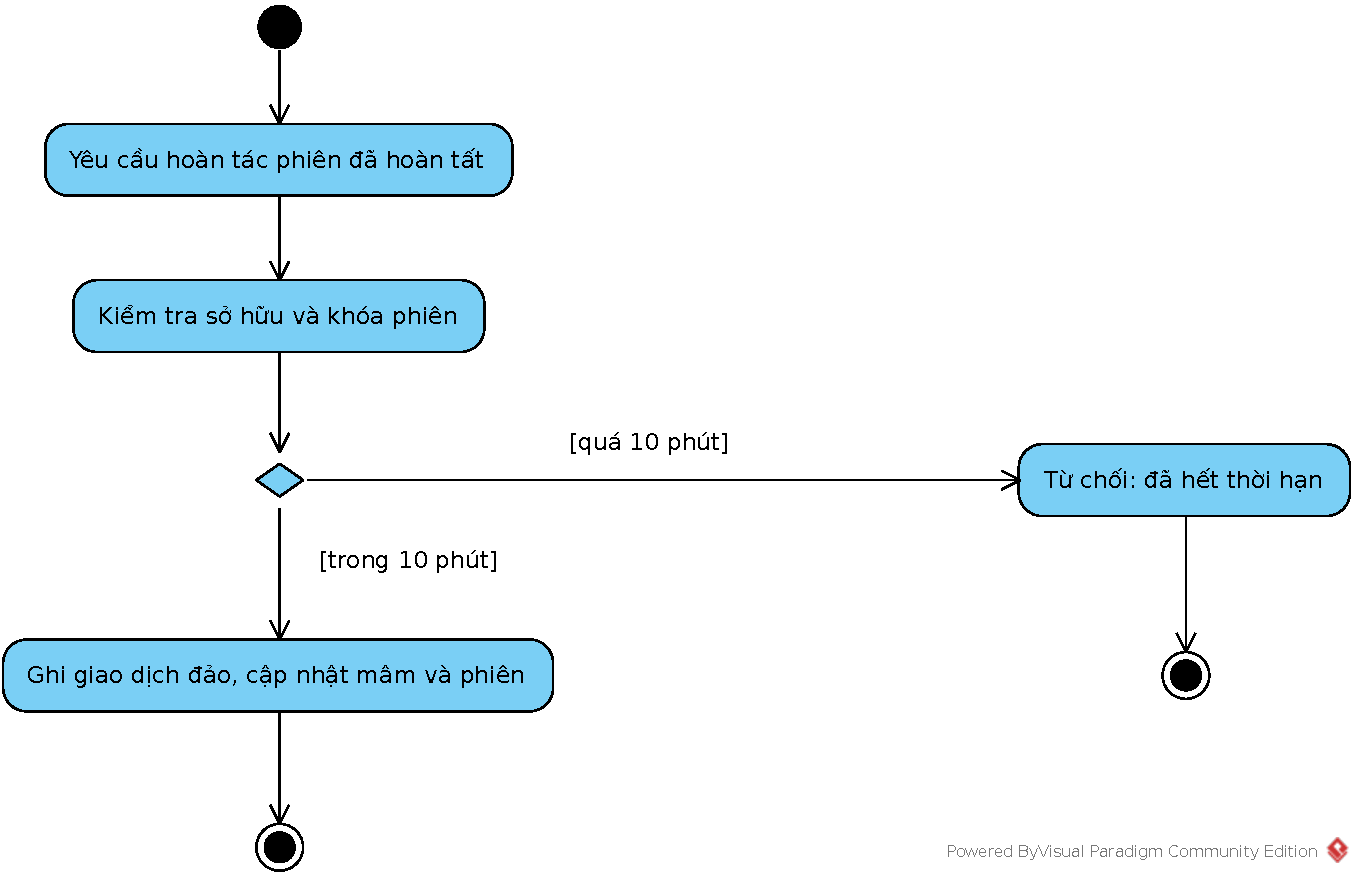
\includegraphics[width=0.96\linewidth,height=0.78\textwidth,keepaspectratio]{assets/AD03.pdf}
\caption{AD03 --- Nhánh nghiệp vụ hoàn tác với tiền điều kiện phiên đã hoàn tất, thuộc người gọi}\label{fig:Bao-cao-Tastoria:5}
\end{figure}
\end{landscape}\clearpage
\subsection{Dữ liệu, mô hình và vận hành}
UC23--UC34. Quy trình gồm khảo sát gu, nhập/\allowbreak{}kiểm tra công thức, cặp thay thế, xuất dữ liệu có quyền sử dụng, đăng ký/\allowbreak{}kiểm định/\allowbreak{}triển khai mô hình, gán nhãn và bảo trì. Tách người biên soạn với người vận hành mô hình; người tham gia khảo sát không trở thành quản trị viên.

\section{Mô hình lớp miền}
Ở pha phân tích, ``Mâm cơm'', ``Món trong mâm'', ``Phiên nấu'' là khái niệm nghiệp vụ. ``Món trong mâm'' cần tách khỏi ``Công thức món'' vì nó mang hệ số khẩu phần, trạng thái thay món và ảnh chụp giá trị ở bữa cụ thể. ``Lô kho'' tách khỏi ``Nguyên liệu'' vì mỗi lô có thời điểm nhập và lượng riêng. Cách tách này tương ứng nguyên tắc phân biệt đối tượng danh mục với dòng giao dịch trong slide.

\begin{figure}[H]\centering
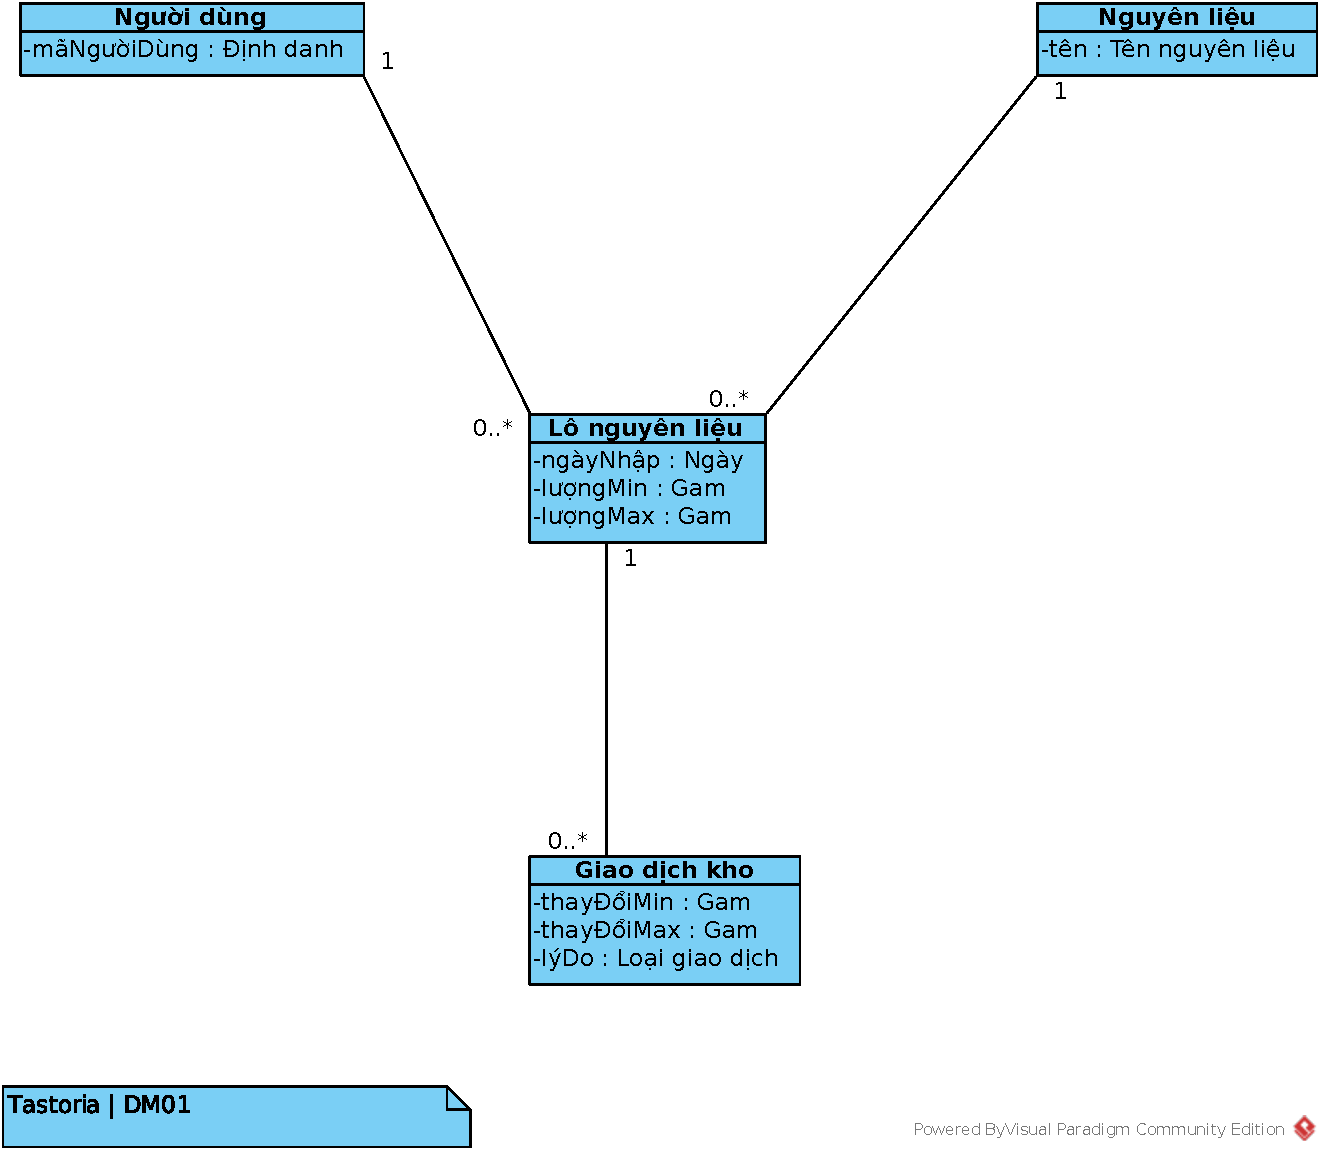
\includegraphics[width=0.96\linewidth,height=0.75\textheight,keepaspectratio]{assets/DM01.pdf}
\caption{DM01 --- Lớp miền kho}\label{fig:Bao-cao-Tastoria:6}
\end{figure}
\clearpage\begin{landscape}
\begin{figure}[H]\centering
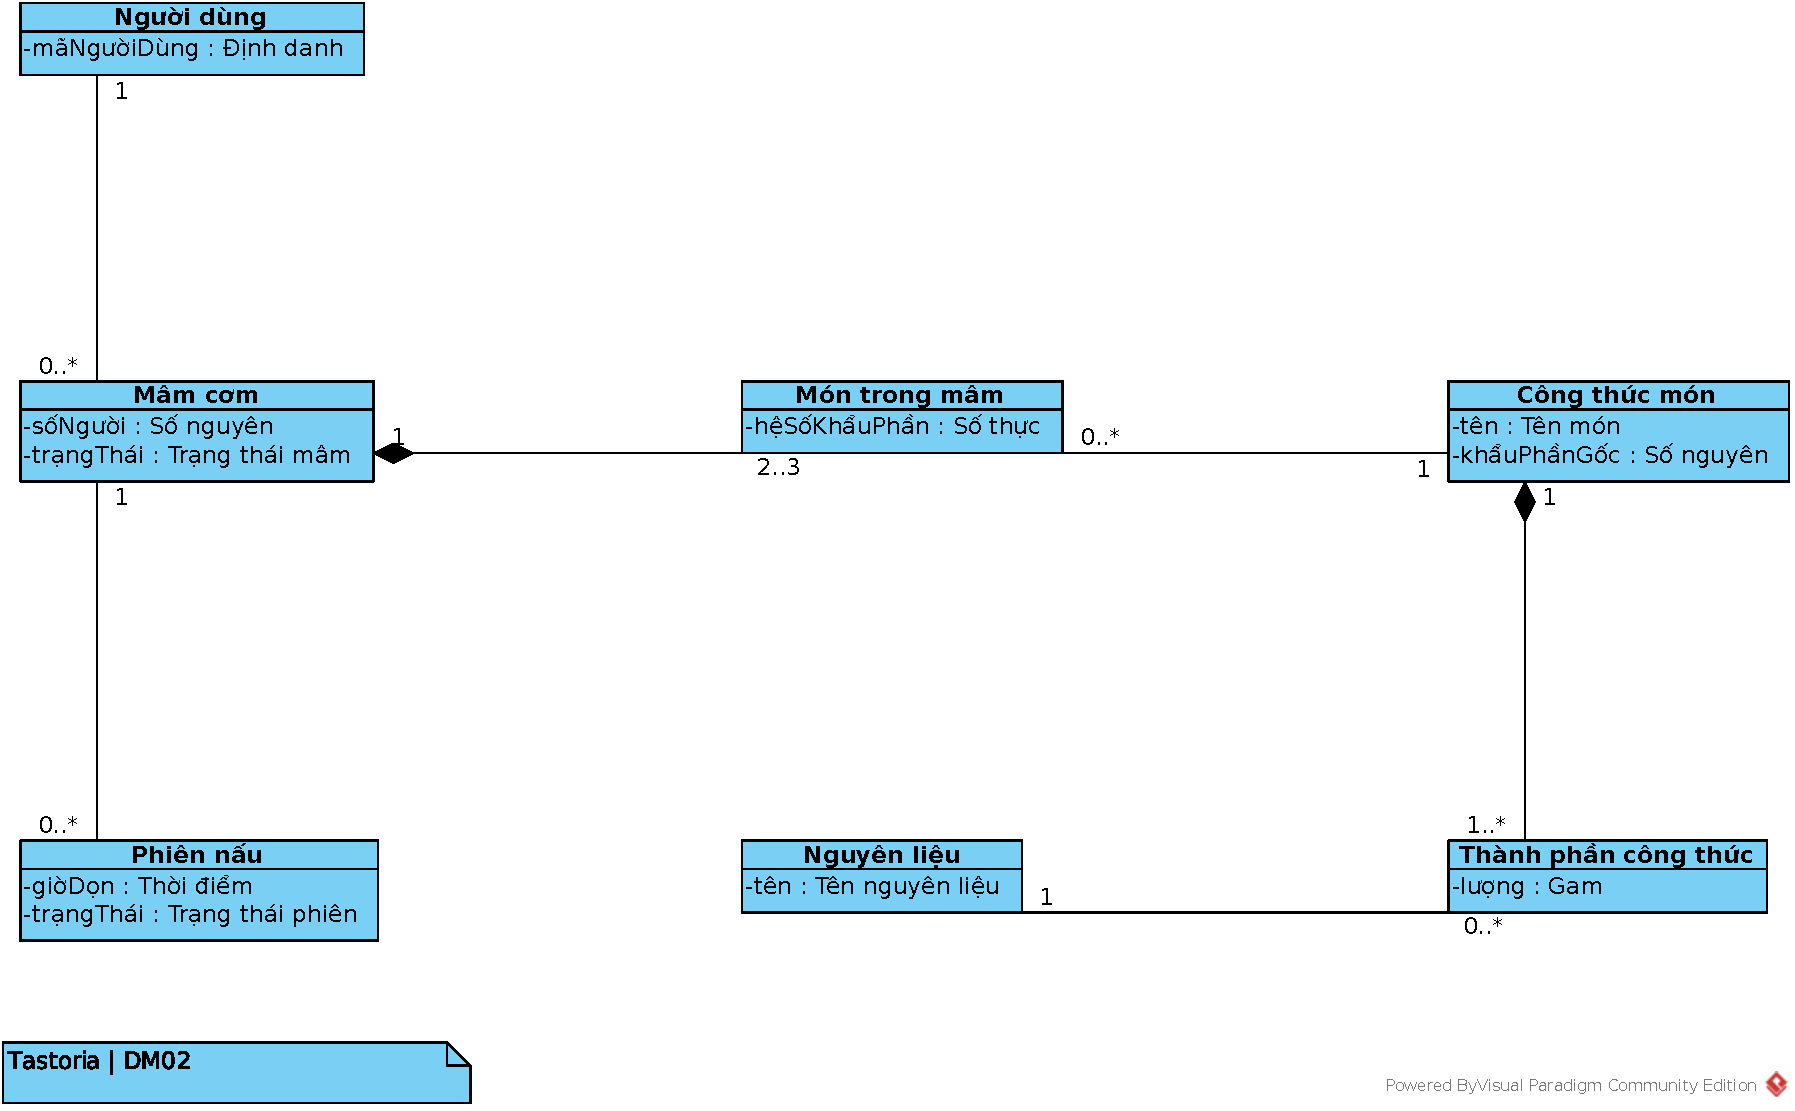
\includegraphics[width=0.96\linewidth,height=0.78\textwidth,keepaspectratio]{assets/DM02.pdf}
\caption{DM02 --- Lớp miền mâm và phiên nấu}\label{fig:Bao-cao-Tastoria:7}
\end{figure}
\end{landscape}\clearpage
Bội số {\small\texttt{2.\allowbreak{}.\allowbreak{}3}} ở DM02 là số \textbf{món active của một mâm hợp lệ} trong mô hình miền rút gọn; bảng vật lý có thể có nhiều dòng hơn để lưu lịch sử đổi. Composition chỉ đặt giữa đối tượng sở hữu và phần tử không có vòng đời độc lập, không đặt giữa người dùng và công thức dùng chung.

{\footnotesize\setlength{\tabcolsep}{0pt}
\begin{longtable}{@{}L{5.133cm}@{\hspace{3mm}}L{5.133cm}@{\hspace{3mm}}L{5.133cm}@{}}
\caption{Mô hình lớp miền}\\
\toprule
\textbf{Quan hệ} & \textbf{Bội số và ý nghĩa} & \textbf{Quyết định mô hình hóa} \\
\midrule\endfirsthead
\multicolumn{3}{l}{\small\itshape Bảng \thetable{} (tiếp theo)}\\
\toprule
\textbf{Quan hệ} & \textbf{Bội số và ý nghĩa} & \textbf{Quyết định mô hình hóa} \\
\midrule\endhead
\bottomrule\endfoot
Người dùng -- Lô nguyên liệu & Một người có 0..* lô; mỗi lô thuộc một người & Association; không suy diễn xóa vật lý dây chuyền từ quyền sở hữu \\ \addlinespace[3pt]
Nguyên liệu -- Lô & Một nguyên liệu được dùng ở 0..* lô; một lô có một nguyên liệu & Danh mục dùng chung có vòng đời độc lập \\ \addlinespace[3pt]
Lô -- Giao dịch kho & Một lô có 0..* giao dịch; mỗi giao dịch chỉ thuộc một lô & Giữ lịch sử, không thay tất cả giao dịch bằng giá trị tổng \\ \addlinespace[3pt]
Mâm -- Món trong mâm & Miền mâm hợp lệ gồm 2..3 món đang hoạt động & Composition của phần tử mâm; DB vẫn giữ thêm dòng đã bị thay \\ \addlinespace[3pt]
Công thức -- Thành phần & Công thức được công bố có 1..* thành phần & Thành phần mang lượng và chỉ có nghĩa trong một công thức \\ \addlinespace[3pt]
Nguyên liệu -- Thành phần & Một nguyên liệu xuất hiện trong nhiều công thức & Association tới danh mục, không composition với danh mục \\ \addlinespace[3pt]
Mâm -- Phiên nấu & Mâm có 0..* phiên theo lịch sử; mỗi phiên thuộc một mâm & ``Tối đa một phiên đang nấu'' là bất biến có điều kiện, không phải bội số lịch sử 0..1 \\ \addlinespace[3pt]
\end{longtable}}
Một quan hệ nhiều--nhiều chỉ có liên kết không đủ để giữ thuộc tính lượng. ``Thành phần công thức'' trở thành đối tượng liên kết giữa công thức và nguyên liệu, mang lượng gam. ``Món trong mâm'' cũng là đối tượng liên kết nhưng cần định danh riêng vì có trạng thái và quan hệ thay thế. Đây là bước chuyển từ quan hệ miền sang bảng nối có thuộc tính, tương ứng phương pháp trong bài PTTKHT.

\section{Lớp phân tích theo use case}
Lớp phân tích được rút ra từ thông tin cần nhớ và trách nhiệm trong UC. Một danh từ xuất hiện trong giao diện chưa chắc là lớp miền: ``nút xác nhận'' thuộc giao diện, ``xác nhận nhập kho'' là hành vi điều phối, còn ``lần quét'' và ``lô nguyên liệu'' có định danh, trạng thái và vòng đời cần lưu. Vì vậy, báo cáo dùng ba nhóm boundary, control và entity để giải thích trách nhiệm trước khi ánh xạ sang mã.

Boundary nhận dữ liệu từ tác nhân và biểu diễn kết quả. Control điều phối một mục tiêu nghiệp vụ, kiểm điều kiện và gọi các đối tượng liên quan. Entity biểu diễn thông tin của miền. Đây là mô hình phân tích, không khẳng định mỗi control phải trở thành một class Python: Tastoria tổ chức phần lớn điều phối bằng module hàm. Các đường \guillemotleft{}use\guillemotright{} trong CL09, CL13, CL15, CL20 và CL30 biểu diễn sử dụng trách nhiệm, không phải khóa ngoại hay quan hệ sở hữu; vì vậy không gán bội số cơ sở dữ liệu cho những đường này.

\subsection{Tài khoản, hồ sơ và quyền dữ liệu}
\clearpage\begin{landscape}
\begin{figure}[H]\centering
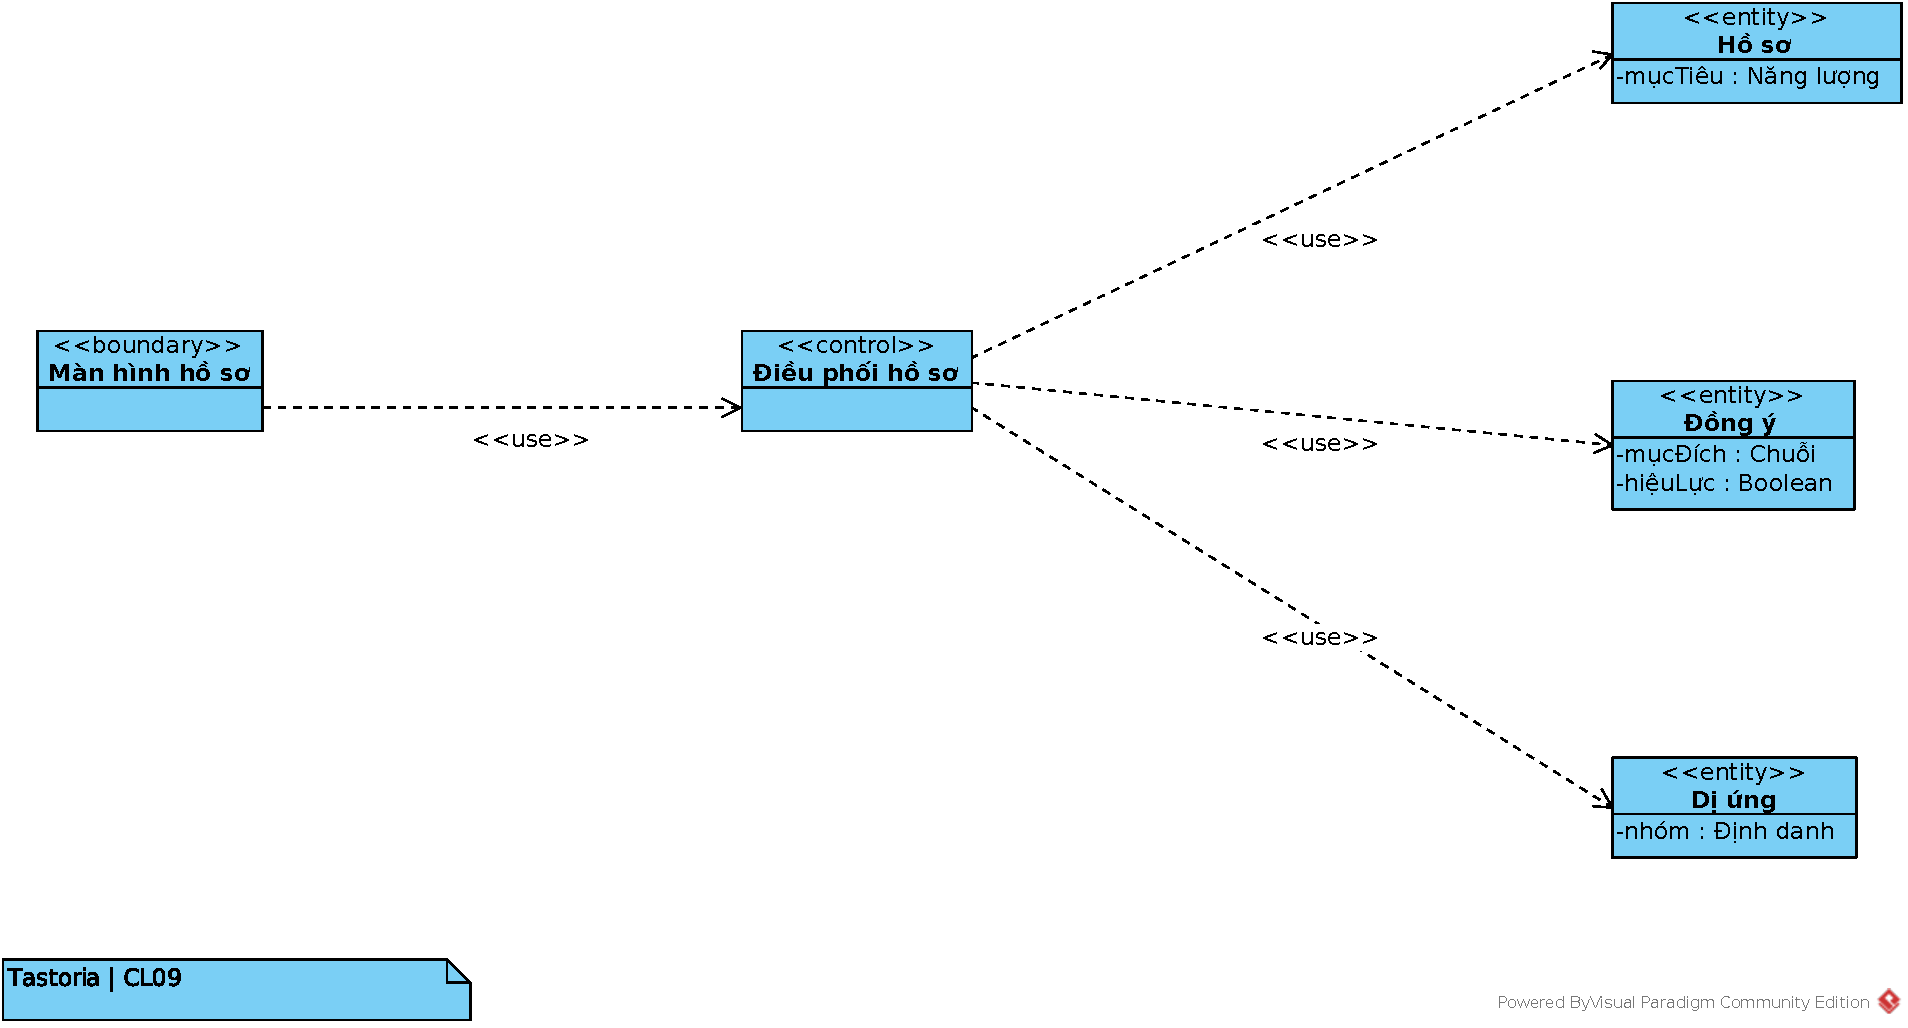
\includegraphics[width=0.96\linewidth,height=0.78\textwidth,keepaspectratio]{assets/CL09.pdf}
\caption{CL09 UC09--10 Hồ sơ và đồng ý}\label{fig:Bao-cao-Tastoria:8}
\end{figure}
\end{landscape}\clearpage
CL09 tách màn hình hồ sơ khỏi điều phối đồng ý và các thực thể hồ sơ/\allowbreak{}dị ứng. Gửi thông tin sức khỏe cần kiểm mục đích xử lý tương ứng; việc đã đăng nhập không thay thế điều kiện này. Khi người dùng bỏ qua phần không bắt buộc, giao diện cần biểu diễn thiếu thông tin, không ghi số 0 như một giá trị đã đo.

\subsection{Quét ảnh và quản lý kho theo lô}
\clearpage\begin{landscape}
\begin{figure}[H]\centering
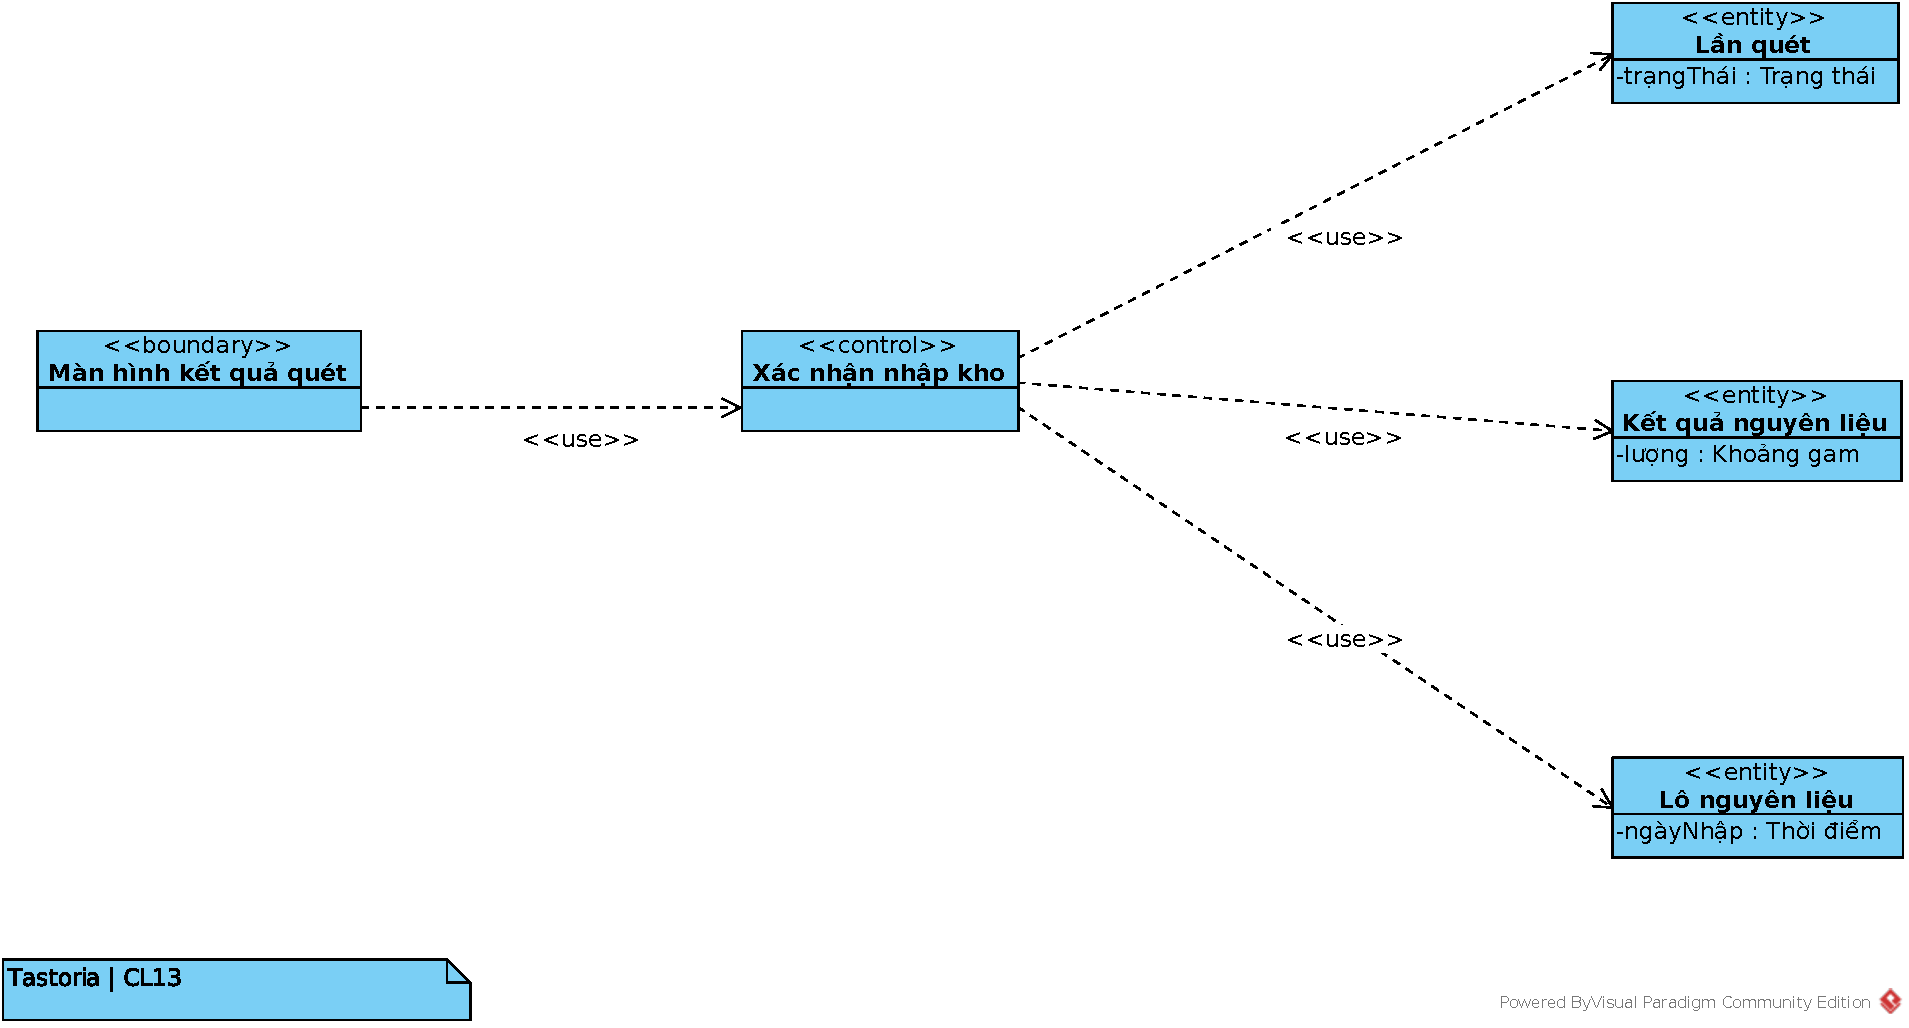
\includegraphics[width=0.96\linewidth,height=0.78\textwidth,keepaspectratio]{assets/CL13.pdf}
\caption{CL13 UC13 Xác nhận kết quả quét}\label{fig:Bao-cao-Tastoria:9}
\end{figure}
\end{landscape}\clearpage
CL13 phân biệt ``kết quả nguyên liệu'' với ``lô nguyên liệu''. Sửa một mục kết quả chưa tạo ra lô; control xác nhận mới chuyển dữ liệu đã duyệt sang nghiệp vụ kho. Quy tắc này giúp người dùng xóa dự đoán sai mà không phải thực hiện một giao dịch xuất kho giả.

\subsection{Gợi ý mâm, đổi món và đi chợ}
\clearpage\begin{landscape}
\begin{figure}[H]\centering
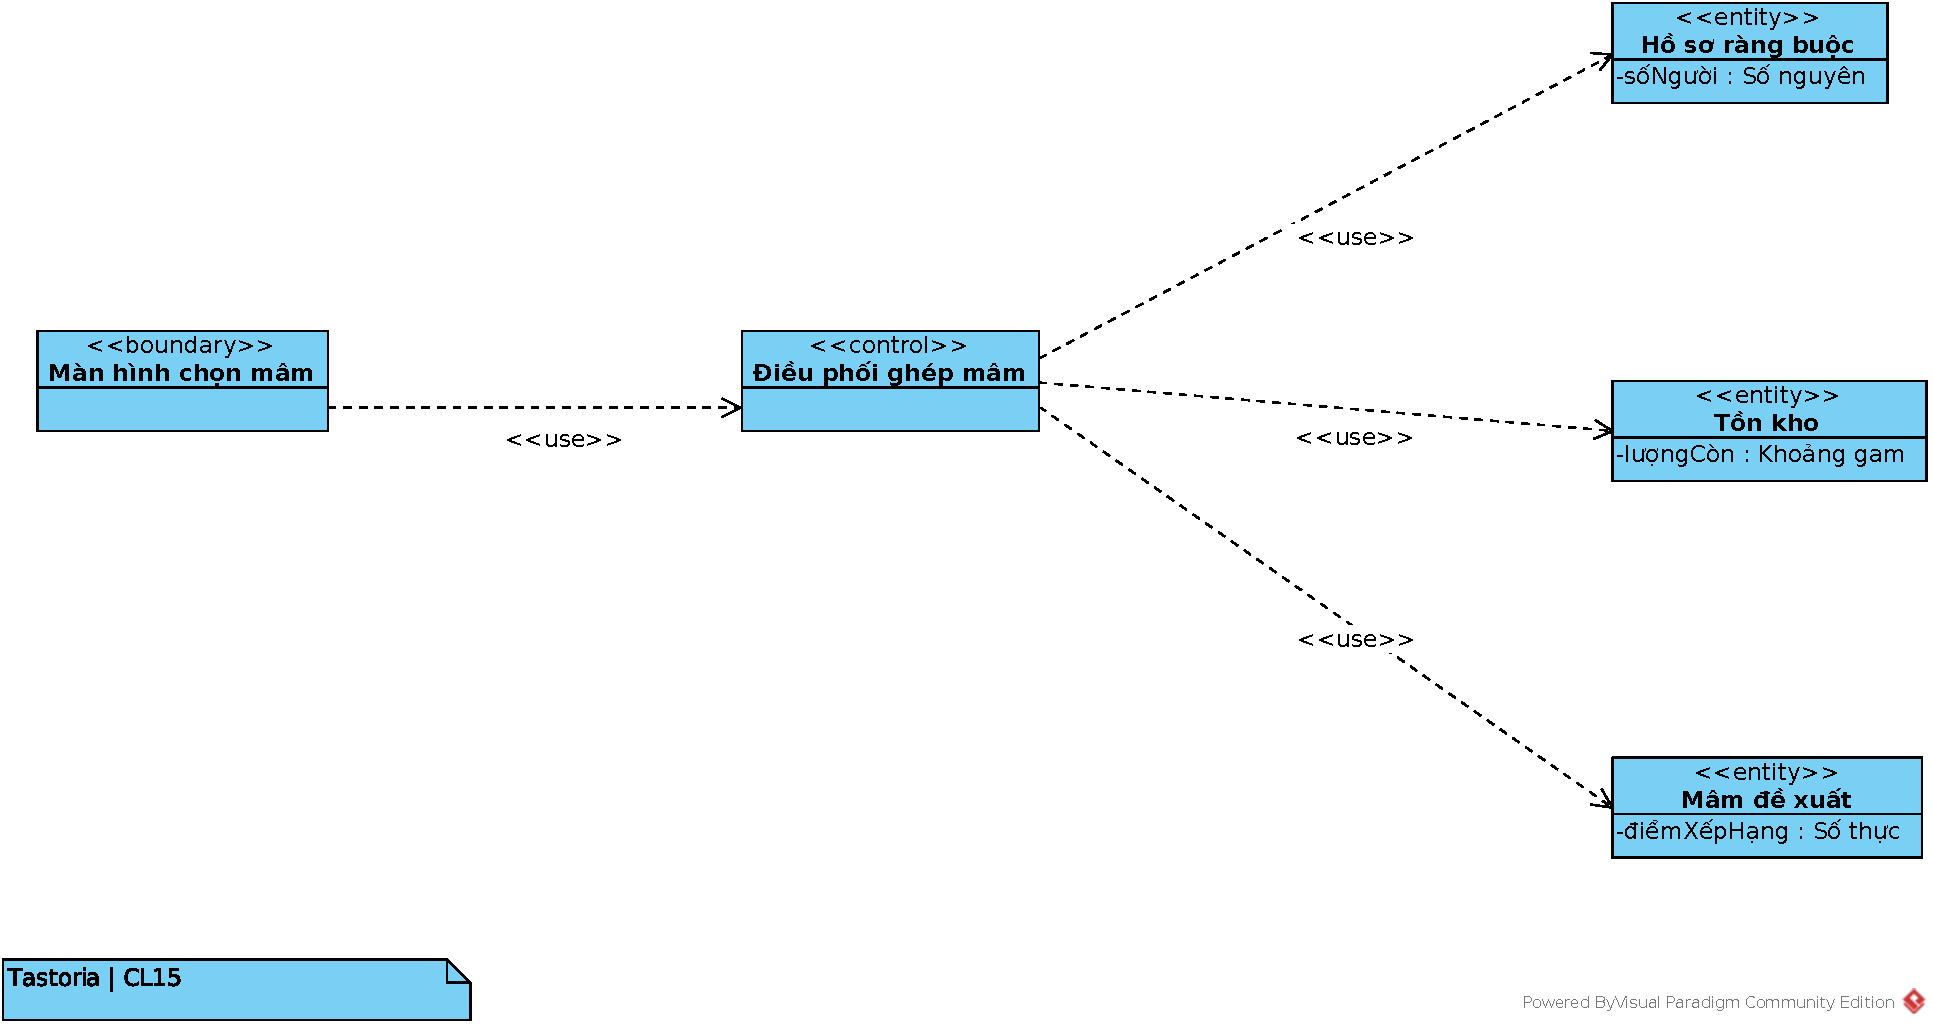
\includegraphics[width=0.96\linewidth,height=0.78\textwidth,keepaspectratio]{assets/CL15.pdf}
\caption{CL15 UC15 Đề xuất mâm cơm}\label{fig:Bao-cao-Tastoria:10}
\end{figure}
\end{landscape}\clearpage
CL15 cho thấy mâm đề xuất phụ thuộc đồng thời hồ sơ ràng buộc và tồn kho. Không để bộ xếp hạng tự quyết định tính hợp lệ: điểm gu cao chỉ giúp sắp thứ tự các phương án đã qua điều kiện bắt buộc.

\subsection{Lịch nấu, hoàn tất, hoàn tác và nhật ký}
\clearpage\begin{landscape}
\begin{figure}[H]\centering
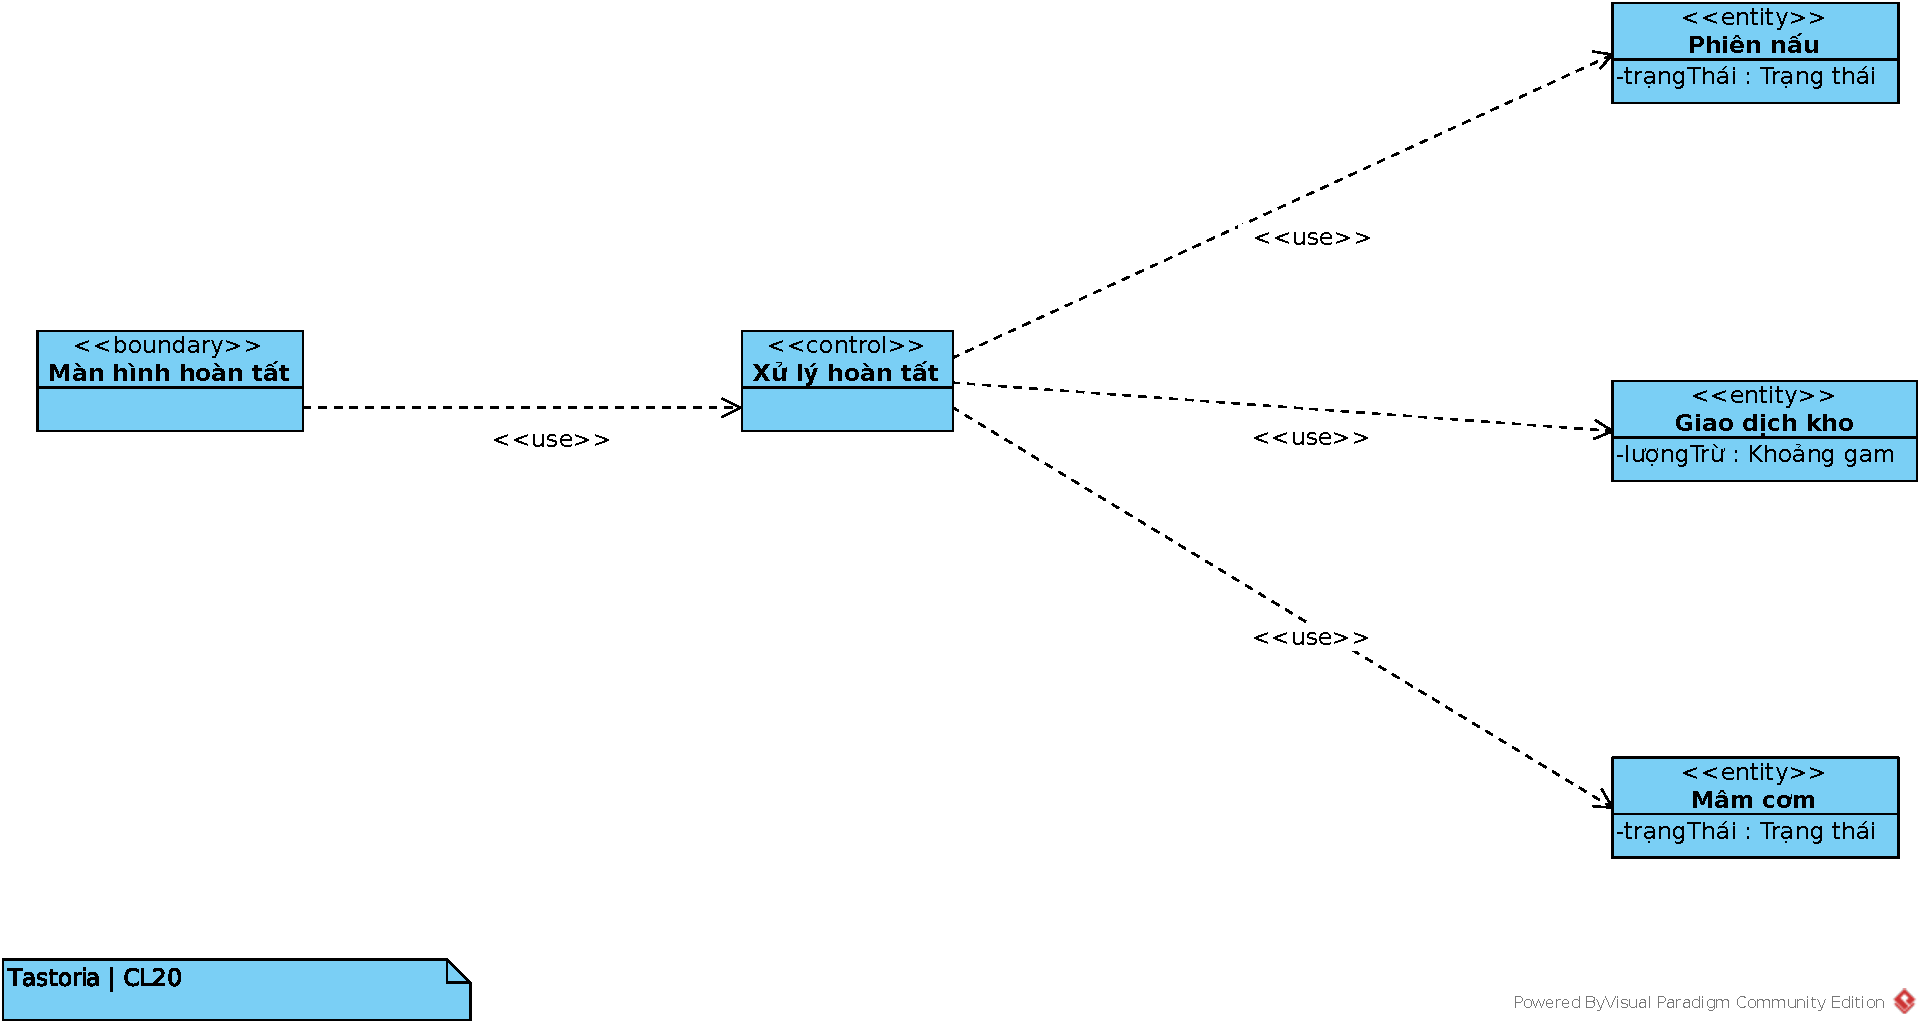
\includegraphics[width=0.96\linewidth,height=0.78\textwidth,keepaspectratio]{assets/CL20.pdf}
\caption{CL20 UC20 Hoàn tất nấu}\label{fig:Bao-cao-Tastoria:11}
\end{figure}
\end{landscape}\clearpage
CL20 đặt xử lý hoàn tất ở control vì thao tác tác động phiên, mâm và giao dịch kho. Không giao toàn bộ nghiệp vụ cho setter trạng thái của phiên. Các dependency tới entity biểu diễn phạm vi trách nhiệm, còn cơ chế khóa và commit được cụ thể hóa ở DS01, SQ01 và SQ02.

\subsection{Dữ liệu, mô hình và vận hành}
\clearpage\begin{landscape}
\begin{figure}[H]\centering
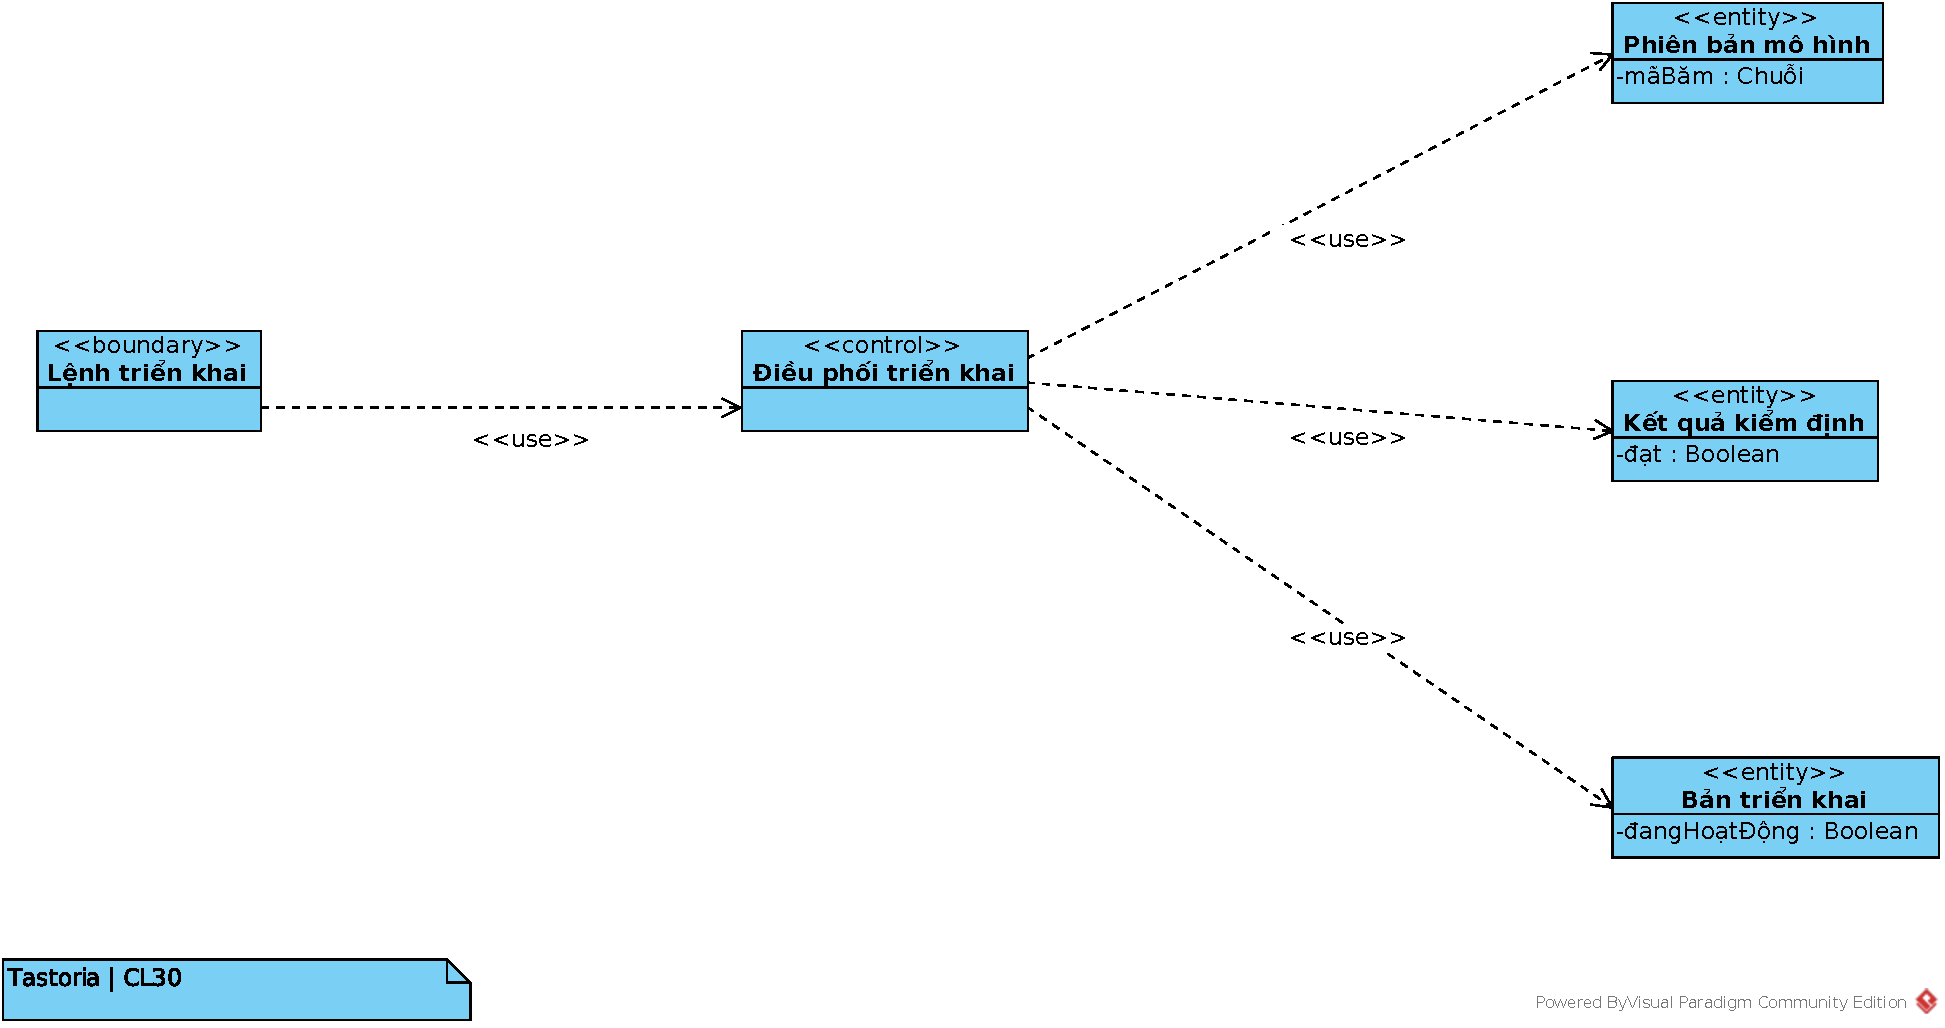
\includegraphics[width=0.96\linewidth,height=0.78\textwidth,keepaspectratio]{assets/CL30.pdf}
\caption{CL30 UC30 Triển khai mô hình}\label{fig:Bao-cao-Tastoria:12}
\end{figure}
\end{landscape}\clearpage
CL30 tách phiên bản, kết quả kiểm định và bản triển khai: một phiên bản có mặt trong kho artifact chưa đồng nghĩa được phục vụ. Control triển khai kiểm quyền và tính phù hợp của phiên bản rồi cập nhật lựa chọn hoạt động. Boundary là lệnh vận hành, không phải một màn hình admin giả định.

\section{Kết quả của pha phân tích}
Đầu ra gồm danh mục 34 UC trong 10 phân hệ, các đặc tả có tiền/\allowbreak{}hậu điều kiện, mô hình miền DM01--DM02 và năm góc nhìn trách nhiệm CL09/\allowbreak{}13/\allowbreak{}15/\allowbreak{}20/\allowbreak{}30. Mô hình miền giải thích quan hệ và bội số; các dependency trong lớp trách nhiệm thể hiện sử dụng, không biểu diễn khóa ngoại. Không yêu cầu mọi UC đều có cùng số loại sơ đồ: mức chi tiết phụ thuộc rủi ro, độ phức tạp và nhu cầu giải thích. Bảng truy vết ở Chương 5 chỉ rõ mô hình nào hỗ trợ mỗi nhóm yêu cầu.
